\documentclass[12pt]{article}
\usepackage[utf8]{inputenc}

\usepackage{lmodern}

\usepackage{enumitem}
\usepackage[margin=2cm]{geometry}

\usepackage{amsmath, amsfonts, amssymb}
\usepackage{graphicx}
%\usepackage{subfigure}
\usepackage{tikz}
\usepackage{pgfplots}
\usepackage{multicol}

\usepackage{comment}
\usepackage{url}
\usepackage{calc}
\usepackage{subcaption}
\usepackage[indent=0pt]{parskip}
\usepackage{animate}

\usepackage{array}
\usepackage{blkarray,booktabs, bigstrut}
\usepackage{bigints}

\pgfplotsset{compat=1.16}

% MATH commands
\newcommand{\ga}{\left\langle}
\newcommand{\da}{\right\rangle}
\newcommand{\oa}{\left\lbrace}
\newcommand{\fa}{\right\rbrace}
\newcommand{\oc}{\left[}
\newcommand{\fc}{\right]}
\newcommand{\op}{\left(}
\newcommand{\fp}{\right)}

\newcommand{\bi}{\mathbf{i}}
\newcommand{\bj}{\mathbf{j}}
\newcommand{\bk}{\mathbf{k}}
\newcommand{\bF}{\mathbf{F}}

\newcommand{\mR}{\mathbb{R}}

\newcommand{\ra}{\rightarrow}
\newcommand{\Ra}{\Rightarrow}

\newcommand{\sech}{\mathrm{sech}\,}
\newcommand{\csch}{\mathrm{csch}\,}
\newcommand{\curl}{\mathrm{curl}\,}
\newcommand{\dive}{\mathrm{div}\,}

\newcommand{\ve}{\varepsilon}
\newcommand{\spc}{\vspace*{0.5cm}}

\DeclareMathOperator{\Ran}{Ran}
\DeclareMathOperator{\Dom}{Dom}

\newcommand{\exo}[1]{\noindent\textcolor{red}{\fbox{\textbf{Problem {#1}}}\hrulefill}\\}
\newcommand{\qu}[4]{\noindent\textcolor{#4}{\fbox{\textbf{Section {#1} | Problem {#2}}} \hrulefill{{\fbox{\textbf{{#3} Points}}}}\\}}

\newcommand{\semester}{Spring 2023}

\newcommand{\CVup}{%
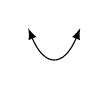
\begin{tikzpicture}
\draw[black, <->, >=latex] (-0.33, 0.5) .. controls (-0.125, 0) and (0.125, 0) .. (0.33, 0.5);
\end{tikzpicture}}

\newcommand{\CVupInc}{%
\begin{tikzpicture}
\draw[black, ->, >=latex] (0,0) .. controls (0.2, 0) and (0.4, 0.2) .. (0.5, 0.5);
\end{tikzpicture}}

\newcommand{\CVupDec}{%
\begin{tikzpicture}[rotate=270]
\draw[black, ->, >=latex] (0,0) .. controls (0.2, 0) and (0.4, 0.2) .. (0.5, 0.5);
\end{tikzpicture}}

\newcommand{\CVdown}{%
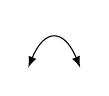
\begin{tikzpicture}
\draw[black, <->, >=latex] (-0.33, -0.5) .. controls (-0.125, 0) and (0.125, 0) .. (0.33, -0.5);
\end{tikzpicture}}

\newcommand{\CVdownInc}{%
\begin{tikzpicture}
\draw[black, ->, >=latex] (-0.5, -0.5) .. controls (-0.5, -0.3) and (-0.5, -0.1) .. (0,0);
\end{tikzpicture}}

\newcommand{\CVdownDec}{%
\begin{tikzpicture}[rotate=-90]
\draw[black, ->, >=latex] (-0.5, -0.5) .. controls (-0.5, -0.3) and (-0.5, -0.1) .. (0,0);
\end{tikzpicture}}

\begin{document}
	\noindent \hrulefill \\
	MATH-241 \hfill Pierre-Olivier Paris{\'e}\\
	Solutions Section 2-5 \hfill \semester \\\vspace*{-1cm}
	
	\noindent\hrulefill
	
	\spc
	
	\exo{8}
	\\
	By the Chain Rule, we have
		\begin{align*}
		F'(x) = 99 (1 + x + x^2)^{98} (1 + 2x) = 99 (1 + 2x) (1 + x + x^2)^{98} .
		\end{align*}
	
	\spc
	
	\exo{10}
	\\
	We have, by the chain rule,
		\begin{align*}
		g'(x) = \frac{3}{2} (2 - \sin x)^{1/2} (-\cos x) = -\frac{3 \cos x \sqrt{2 - \sin x}}{2} .
		\end{align*}
	
	\spc
	
	\exo{11}
	\\
	The outer function is $f(t) = \frac{1}{t^2}$ and the inside function is $g(t) = \cos t + \tan t$. This implies that 
		\begin{align*}
		A (t) = f (g (t)) .
		\end{align*} 
	Using the Chain Rule, we have
		\begin{align*}
		A' (t) = f' (g (t)) g' (t) .
		\end{align*}
	Now, we have
		\begin{align*}
		f'(t) = (t^{-2})' = -2 t^{-3} = -\frac{2}{t^3} .
		\end{align*}
	Also, we have
		\begin{align*}
		g' (t) = -\sin t + \sec^2 t
		\end{align*}
	and therefore
		\begin{align*}
		A' (t) &= -\frac{2}{(\cos t + \tan t)^3} (-\sin t + \sec^2 t)  \\
		&= - 2\frac{\sec^2 t - \sin t}{(\cos t + \tan t)^3} .
		\end{align*}
		
	\spc
	
	\exo{30}
	\\
	We use the chaine rule and we get
		\begin{align*}
		ds/dt = \frac{1}{2} \Big( \frac{1 + \sin t}{1 + \cos t} \Big)^{-1/2} \frac{d}{dx} \Big( \frac{1 + \sin t}{1 + \cos t} \Big) .
		\end{align*}
	The derivative of $(1 +\sin t)/(1 + \cos t)$ is
		\begin{align*}
		\frac{\cos t (1 + \cos t) - (1 + \sin t) (-\sin t)}{(1 + \cos t)^2} = \frac{\cos t + \cos^2 t + \sin t + \sin^2 t}{(1 + \cos t)^2} = \frac{1 + \sin t + \cos t}{(1 + \cos t)^2} .
		\end{align*}
	Thus, the final answer looks like
		\begin{align*}
		ds/dt = \frac{1 + \sin t + \cos t}{2 (1 + \cos t)^{3/2} \sqrt{1 + \sin t}} .
		\end{align*}
	
	
\end{document}